\section{Approach}

\begin{figure}
    \centering
    
\includegraphics[width=1\columnwidth]{figs/overview.pdf}
    \caption{Overview of \tech}
    \label{fig:overview}
\end{figure}

\tech is a live, self-evolving agent that improves and expands its capabilities \textit{on the fly} while solving an issue. 
Our key insight is recognizing that agents themselves can be iteratively improved, just like the software issues they are designed to solve.
The space in which an agent can evolve includes not only the tools it uses but also the underlying agent scaffold itself.
In this work, we start from a simple agent scaffold and focus primarily on self-evolution for tool creation and usage, as tools represent one of the most critical components of an agent.
We now describe how \tech provides a framework for \llm{s} to develop and use their own tools on the fly. 



Figure~\ref{fig:overview} presents an overview of \tech{}.
First, \circled{1} we take in both the project codebase and the description of the issue to be solved. 
We then provide this information to the agent and initialize it with a set of tools.
In the beginning, the agent may only have access to a limited set of tools (e.g., bash commands) and the goal of \tech is to allow the agent to generate and use its own tools \textit{on the fly} while solving the issue.
As the agent is solving the issue, at each step,{it} can choose to either \circled{2} output a command (e.g., to use a tool) or \circled{3} create a custom tool that can help it solve the issue.
In \tech, we define a custom tool as a script that can be executed in the environment. 
This provides an intuitive and straightforward tool-usage interface for the agent, allowing it to output a command to use any custom tool.
Next, different from existing approaches that \circled{4} directly provide the environmental feedback output to the agent, \circled{5} we specifically ask the agent to reflect upon the past steps and decide whether a tool should be created in the feedback message.
This loop is repeated until the agent has submitted a solution \circled{6} to the initial problem.
Unlike prior agentic setups where the set of tools and possible actions available to the agent is fixed, \tech allows the agent to perform live self-evolution by creating and using custom tools on the fly.




\subsection{On-the-fly Self Evolution}

The key idea of \tech is to enable the agent self-improve by modifying its{ own scaffold}{, such as} creating custom tools based on the problem and previous trajectories.
To support tool creation, we apply several simple modifications to the initial prompt of the agent.
Specifically, we provide instructions and examples illustrating how a tool should be created and used.
More importantly, we indicate to the agent that: (1) the goal of any tools it creates should be to help it better solve the tasks and (2) the created tools can be for any purpose and do not need to be general. 

In addition to introducing the ability for agents to create tools through the initial prompt, we also explicitly ask the agent to reflect on its past trajectory to determine if it should create any tools after each step. 
This is done by appending a simple reflection message after each environmental feedback.
In our experiments, we found that this reflection process is necessary to remind the agents to design tools that are useful and specific for the particular issue.

It is important to point out that the modifications made to a regular agentic framework by \tech are extremely simple (See Appendix~\ref{appendix:initial_prompt} for both the initial prompt and reflection message).
\tech does not make any changes to the agentic loop, impose a particular workflow, or require any costly offline training.
Instead, the focus is on allowing and extending the ability for agents to create their own custom tools at runtime to improve performance and reduce manual tool-creation effort.
This allows \tech to be extremely general and applicable across a wide-range of different tasks, \llm{s}, and agent scaffolds. 
Furthermore, we also note that software agents, in essence, are also software.
As such, they can be modified and updated on the fly by software agents (themselves) no different than any other software repository.
In \tech, we leverage this insight for on-the-fly self-improvement by enabling the agents to create their own custom tools depending on the problem at hand.
We next describe the custom tools agents create in more detail.


\subsection{Custom Tool Synthesis}

In \tech, we define a custom tool as a script that can be executed in the environment.
This allows the agents to both easily create tools (by creating a script file) and use the created tools (by running the script with arguments).
We believe this is a general and intuitive interface that is suitable for a wide range of tasks.


\parabf{Example editing tool.} Figure~\ref{fig:example_tools} shows an example of a custom tool created by the agent. 
This is an editing tool that allows the agent to edit a file by replacing, inserting, or deleting code.
We see that it contains the necessary tool logic as well as clear instructions on how the tool can be used.
Compared with bash commands which can potentially overwhelm the agent with many different arguments and flags, the tools that agents create themselves have a straightforward purpose and are easy to use.
Furthermore, in the example, we see that the editing tool also provides relevant feedback messages such as indicating whether the replacement edit was successful or not.
This feedback can be critically important to inform the next actions taken by the agents.
On the other hand, a bash editing command like \CodeIn{sed} does not indicate the result of the edit such that a replacement operation where the string to be replaced does not exist will produce no warning message but still return a success code.
As such, the agent may be misguided into thinking that the edit was successful when, in fact, no changes have been made to the file.

\tech also encourages agents to create tools that can improve the efficiency of their workflows. 
For example, a common step in solving an issue is to identify the locations of relevant code snippets in order to understand the root cause.
In this case, a custom search tool can be useful for searching code within certain directories and displaying their surrounding context.
While it is possible to achieve the same outcome of a custom search tool using a combination of different bash commands (e.g., \CodeIn{grep}, \CodeIn{find}, \CodeIn{cat}), the agent often needs to take multiple steps to perform the actual search, leading to increased context length and time required to solve an issue.
By creating custom tools that can handle complex and multi-step tasks, \tech can improve both the effectiveness and efficiency of agents.

\begin{wrapfigure}{r}{0.4\textwidth}
  \begin{minipage}{\linewidth}
  \centering
  \captionsetup[subfigure]{justification=centering}
  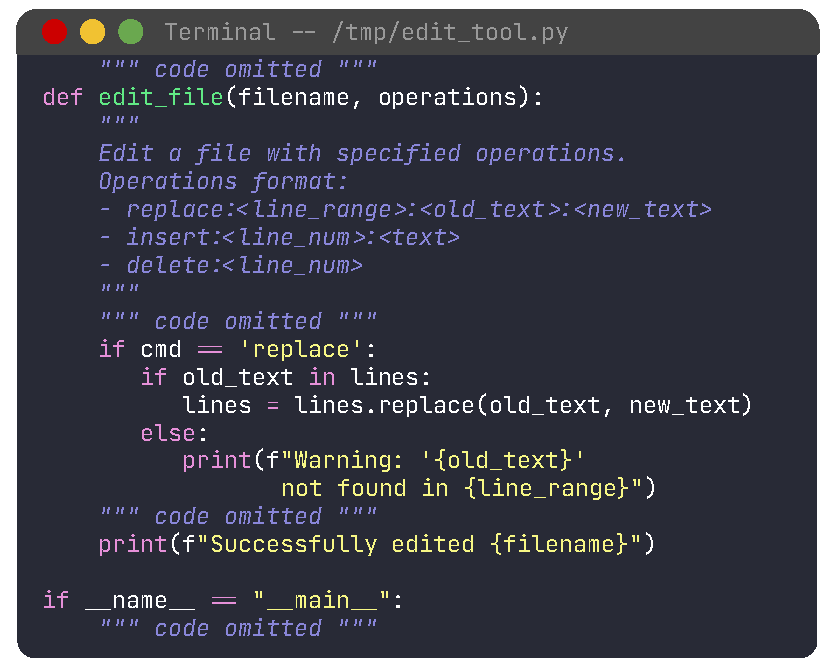
\includegraphics[width=\linewidth]{figs/example_tools.pdf}
  \subcaption{Edit tool}
  \label{fig:example_tools}
  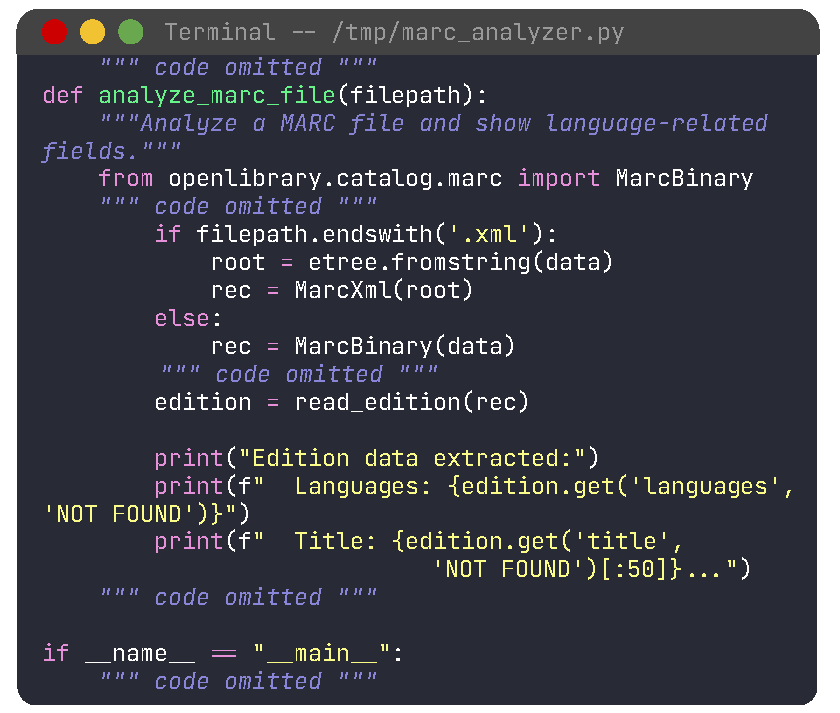
\includegraphics[width=\linewidth]{figs/example_tools_2.pdf}
  \subcaption{\CodeIn{MARC} file analyzer tool}
  \label{fig:example_tools2}
  \end{minipage}
  \caption{Example custom tools}
  \label{fig:example_tool_large_1}
\end{wrapfigure}

\textbf{Example issue-specific tool.}
In addition to general tools, another benefit of \tech is its ability to create issue-specific tools.
Figure~\ref{fig:example_tools2} shows an example of a custom tool that is specifically tailored to a particular issue.
In this example, the tool analyzes \CodeIn{MARC} files, a file format for publication or text records, and prints them in a human-readable format. 
The agent can create this tool and use it to display the content of relevant \CodeIn{MARC} files (including binary files) that serve as test cases, helping it better understand the issue and evaluate potential patches.
Such functionality cannot be achieved easily using simple bash commands or even general-purpose tools.
By enabling the agents to create arbitrary custom tools on the fly, \tech can generate specialized tools for individual problems, allowing it to solve issues more effectively.



A fair question to ask is \textit{why not generate these tools directly in the beginning?} 
The reason is that tool creation, similar to manual problem solving, is also an iterative process.
We need to understand the problem at hand and during the solving process identify the issues in order to come up with helpful tools in different scenarios.
For example, in the \CodeIn{MARC} file example, it is not immediately obvious that we need to create a custom tool specifically to analyze \CodeIn{MARC} files.
By creating all the tools in the beginning and applying this fixed set of tools during the entire process, we will lose the opportunity to design custom tools that are helpful in unique situations.
Additionally, having access to all possible tools are not necessarily better as they can overwhelm and mislead the agent.
Furthermore, the agent may often iterate on or modify the tools it has created which requires runtime modification abilities not available under a fixed tool setup. 
\tech provides the ability for agents to automatically synthesize customs tools on the fly without any additional overhead from heavy scaffold modifications or costly offline training updates.
